\chapter{Analisi delle Prestazioni e Affidabilità dei Protocolli}

\section{Introduzione}

Nel contesto della domotica residenziale, la selezione del protocollo di comunicazione rappresenta un passaggio cruciale, capace di incidere in modo determinante sulle prestazioni complessive del sistema, sull’affidabilità delle connessioni tra i dispositivi e, non da ultimo, sull’esperienza d’uso percepita dagli utenti finali. Questo capitolo si propone di esplorare in modo approfondito le caratteristiche tecniche e operative dei principali protocolli IoT impiegati in ambito domestico, offrendo strumenti concreti per orientare la scelta verso la soluzione più adeguata in funzione delle specifiche esigenze progettuali.\\

L’evoluzione tecnologica degli ultimi anni ha favorito la diffusione di una molteplicità di protocolli, ciascuno sviluppato per rispondere a determinati requisiti funzionali o vincoli strutturali. Nessuno di essi può essere considerato intrinsecamente “migliore” in senso assoluto: la decisione finale deve necessariamente derivare da un’attenta analisi comparativa, che tenga conto di fattori quali la scalabilità, il consumo energetico, la latenza, la sicurezza, la compatibilità con ecosistemi preesistenti e il grado di complessità richiesto per l’integrazione.

\section{Indicatori chiave di performance}

Per capire davvero quanto un protocollo di comunicazione IoT sia efficace all’interno di un’abitazione intelligente, non basta leggerne le specifiche tecniche ma è fondamentale considerare alcuni indicatori chiave di performance, definiti con il nome Key Performance Indicators abbreviato in  (KPI), questi indicatori oggettivi ci  aiutano a valutare in modo concreto e comparabile il comportamento di ciascuna tecnologia nelle situazioni reali di abitazioni comuni.

\subsection{Latenza: il tempo di risposta del sistema}

Uno degli aspetti che più influisce sull’esperienza d’uso quotidiana è la \textbf{latenza}, ovvero il tempo che passa tra l’invio di un comando e la sua esecuzione. In altre parole, quanto velocemente la casa “risponde” quando chiediamo qualcosa. È un po’ come premere l’interruttore della luce: se dopo averlo fatto ci vogliono più di 200-300 millisecondi perché la lampada si accenda, la sensazione immediata è che qualcosa non funzioni a dovere – anche se tecnicamente tutto è sotto controllo. Questo breve ritardo può sembrare irrilevante, ma oltre una certa soglia diventa fastidioso e può minare la fiducia nel sistema.\\

Naturalmente, non tutti i protocolli si comportano allo stesso modo. \textbf{Zigbee}, ad esempio, è generalmente molto reattivo nelle comunicazioni dirette, con latenze comprese tra i 15 e i 30 millisecondi. Tuttavia, quando la rete diventa più complessa, come nel caso di una struttura mesh con più passaggi intermedi (i cosiddetti multi-hop), il tempo di risposta può allungarsi fino a 50-100 millisecondi.\\

Il \textbf{Wi-Fi}, se ottimizzato per applicazioni in tempo reale, può offrire prestazioni ancora migliori, arrivando a latenze inferiori ai 10 millisecondi. Ma c’è un prezzo da pagare: questi risultati richiedono un consumo energetico decisamente più elevato, rendendo il Wi-Fi meno adatto per dispositivi alimentati a batteria, come sensori o piccoli attuatori che devono funzionare per anni senza manutenzione.\\

In definitiva, la scelta del protocollo deve sempre tenere conto di un equilibrio tra velocità, efficienza energetica e caratteristiche dell’ambiente domestico in cui verrà implementato. La reattività è importante, ma lo è altrettanto la capacità del sistema di durare nel tempo senza interventi continui.


\subsection{Consumo energetico: la sfida dell’autonomia}

Tra le principali sfide dell’Internet of Things applicato alla domotica, il consumo energetico occupa un ruolo di primo piano. In particolare, numerosi dispositivi domestici, come sensori di movimento, di temperatura, o di apertura porte e finestre, devono poter funzionare per lunghi periodi, spesso per anni, con una singola batteria di piccole dimensioni. In questo scenario, l’efficienza energetica non rappresenta solo un vantaggio, ma un requisito fondamentale per garantire la sostenibilità e l’affidabilità dell’intero ecosistema smart.

I protocolli di comunicazione IoT si distinguono nettamente per quanto riguarda l’impatto energetico, in funzione del loro design, delle modalità di trasmissione e della gestione dei cicli di attività e standby. Di seguito, una panoramica comparativa delle principali soluzioni:

\begin{itemize}
    \item \textbf{Z-Wave}: Progettato fin dalle origini per applicazioni a basso consumo, Z-Wave offre consumi estremamente contenuti in modalità standby (inferiori a 1 µA) e una richiesta energetica in trasmissione intorno ai 30–40 mA, limitata a brevi istanti. Queste caratteristiche lo rendono ideale per dispositivi alimentati a batteria.
   \item \textbf{Zigbee}: Anch’esso particolarmente efficiente, Zigbee utilizza modalità “sleep” avanzate con assorbimenti inferiori ai 3 µA. Il tempo di riattivazione è molto contenuto (meno di 15 ms), garantendo un buon compromesso tra reattività e risparmio energetico.

    \item \textbf{Thread}: Questo protocollo eredita l’approccio efficiente di Zigbee, ma introduce ulteriori ottimizzazioni per supportare il routing basato su IPv6, consentendo una gestione energetica ancora più flessibile e scalabile, pur mantenendo consumi contenuti.

    \item \textbf{Wi-Fi}: Tradizionalmente meno adatto ai dispositivi a basso consumo, anche nelle sue versioni più recenti – come Wi-Fi 6 – continua a presentare assorbimenti elevati, con consumi in standby nell’ordine dei millesimi di ampere (mA), decisamente superiori rispetto agli standard sopra citati.
\end{itemize}

Per rendere il confronto più concreto, si consideri un sensore di temperatura basato su Z-Wave, configurato per trasmettere dati ogni 5 minuti: in condizioni ottimali, può operare per un periodo compreso tra i 5 e i 7 anni con una singola batteria tipo CR2032. Al contrario, un dispositivo Wi-Fi equivalente richiederebbe una ricarica mensile o un’alimentazione continua, fattore che limita fortemente la sua applicabilità in scenari stand-alone.

\subsection{Larghezza di banda: quanto possono davvero ``parlare'' i dispositivi}

Un altro parametro importante da considerare, soprattutto in certi scenari, è la \textbf{larghezza di banda}, ovvero la quantità di dati che possono essere trasmessi attraverso la rete in un dato intervallo di tempo. Anche se molti dispositivi domotici scambiano solo piccoli pacchetti di dati (ad esempio, un comando on/off o la lettura di un sensore), esistono casi d’uso che richiedono una capacità di trasferimento ben più ampia.

Alcuni esempi includono:

\begin{itemize}
    \item Lo \textit{streaming video} in tempo reale da telecamere di sicurezza
    \item Gli \textit{aggiornamenti firmware over-the-air}, fondamentali per la manutenzione remota
    \item Il trasferimento di \textit{log diagnostici} da dispositivi complessi
    \item Il controllo e la sincronizzazione di \textit{impianti audio multi-room}
\end{itemize}

In questi contesti, la banda disponibile fa la differenza. I protocolli IoT presentano valori molto diversi in termini di velocità massima e throughput reale, come evidenziato nella tabella seguente:

\begin{table}[h]
\centering
\begin{tabular}{|l|c|c|}
\hline
\textbf{Protocollo} & \textbf{Velocità massima} & \textbf{Throughput reale stimato} \\
\hline
Z-Wave & 100 kbps & 40–60 kbps \\
Zigbee & 250 kbps & 100–150 kbps \\
Thread & 250 kbps & 100–150 kbps \\
Wi-Fi 4 & 600 Mbps & 100–200 Mbps \\
Wi-Fi 6 & 9.6 Gbps & 1–2 Gbps \\
\hline
\end{tabular}
\caption{Confronto tra velocità teoriche e throughput pratico dei principali protocolli IoT}
\end{table}

Come si osserva, \textbf{Wi-Fi} domina nettamente per capacità di banda. Tuttavia, nella maggior parte degli impianti domotici, questa potenza risulta sovradimensionata: un semplice comando per accendere una luce o inviare una lettura della temperatura richiede pochi byte, rendendo il Wi-Fi inefficiente in termini energetici per compiti così semplici \cite{wifi6-spec}. 

In altre parole, usare il Wi-Fi per trasmettere dati minimi è come utilizzare un camion per consegnare una cartolina: funziona, ma è chiaramente uno spreco.

\vspace{0.5cm}

\subsection{Affidabilità e resilienza: quando la rete deve sapersela cavare da sola}

Perché un sistema domotico possa davvero definirsi affidabile, non basta che funzioni “quando tutto va bene”: deve essere in grado di reagire e adattarsi anche quando qualcosa non va come previsto. È in queste situazioni che entrano in gioco due concetti fondamentali: \textbf{affidabilità} e \textbf{resilienza}.

In termini pratici, un protocollo di comunicazione deve possedere alcune capacità essenziali:

\begin{itemize}
    \item \textbf{Gestione delle interferenze}: saper mantenere la comunicazione anche in ambienti ricchi di segnali wireless (Wi-Fi, Bluetooth, ecc.)
    \item \textbf{Ritrasmissione automatica}: garantire che i pacchetti persi vengano inviati di nuovo senza necessità di intervento
    \item \textbf{Routing dinamico}: trovare percorsi alternativi se un nodo della rete diventa inattivo o instabile
    \item \textbf{Prioritizzazione del traffico}: assegnare maggiore importanza ai messaggi critici tramite meccanismi di \textit{Quality of Service} (QoS)
\end{itemize}

Le reti \textit{mesh} basate su \textbf{Zigbee} e \textbf{Thread} sono progettate proprio per affrontare queste sfide: grazie ad algoritmi di routing intelligente, sono in grado di riorganizzarsi in autonomia e reindirizzare i messaggi qualora un dispositivo venga rimosso, sostituito o risulti non raggiungibile \cite{zigbee-spec,thread-spec}. Questo approccio rende il sistema più flessibile e robusto nel tempo.\\

Anche \textbf{Z-Wave}, pur avendo una struttura mesh meno estesa, offre un vantaggio rilevante: opera su frequenze \textbf{sub-GHz}, in particolare intorno agli 868 MHz in Europa, una banda meno affollata rispetto alla classica 2.4 GHz utilizzata da molti altri protocolli. Ciò si traduce in una maggiore immunità alle interferenze, che spesso rappresentano un problema negli ambienti domestici saturi di dispositivi wireless \cite{zwave-spec}.\\

Per quanto riguarda il \textbf{Wi-Fi}, nonostante la sua ampia diffusione e le elevate prestazioni in termini di velocità, si dimostra talvolta meno resiliente in ambienti particolarmente congestionati. La stabilità complessiva della rete Wi-Fi dipende fortemente dalla qualità dell'infrastruttura (router, access point, gestione dei canali), e in caso di sovraccarico o malfunzionamenti può mostrare latenze elevate o perdita di pacchetti \cite{wifi6-spec}.\\

Come illustrato nella Figura~\ref{fig:smart-home-mesh-vs-wifi}, le reti mesh consentono a ogni nodo di fungere da ponte per altri dispositivi, garantendo comunicazione anche in caso di guasti o disconnessioni.

\begin{comment}

\begin{figure}[h!]
    \centering
    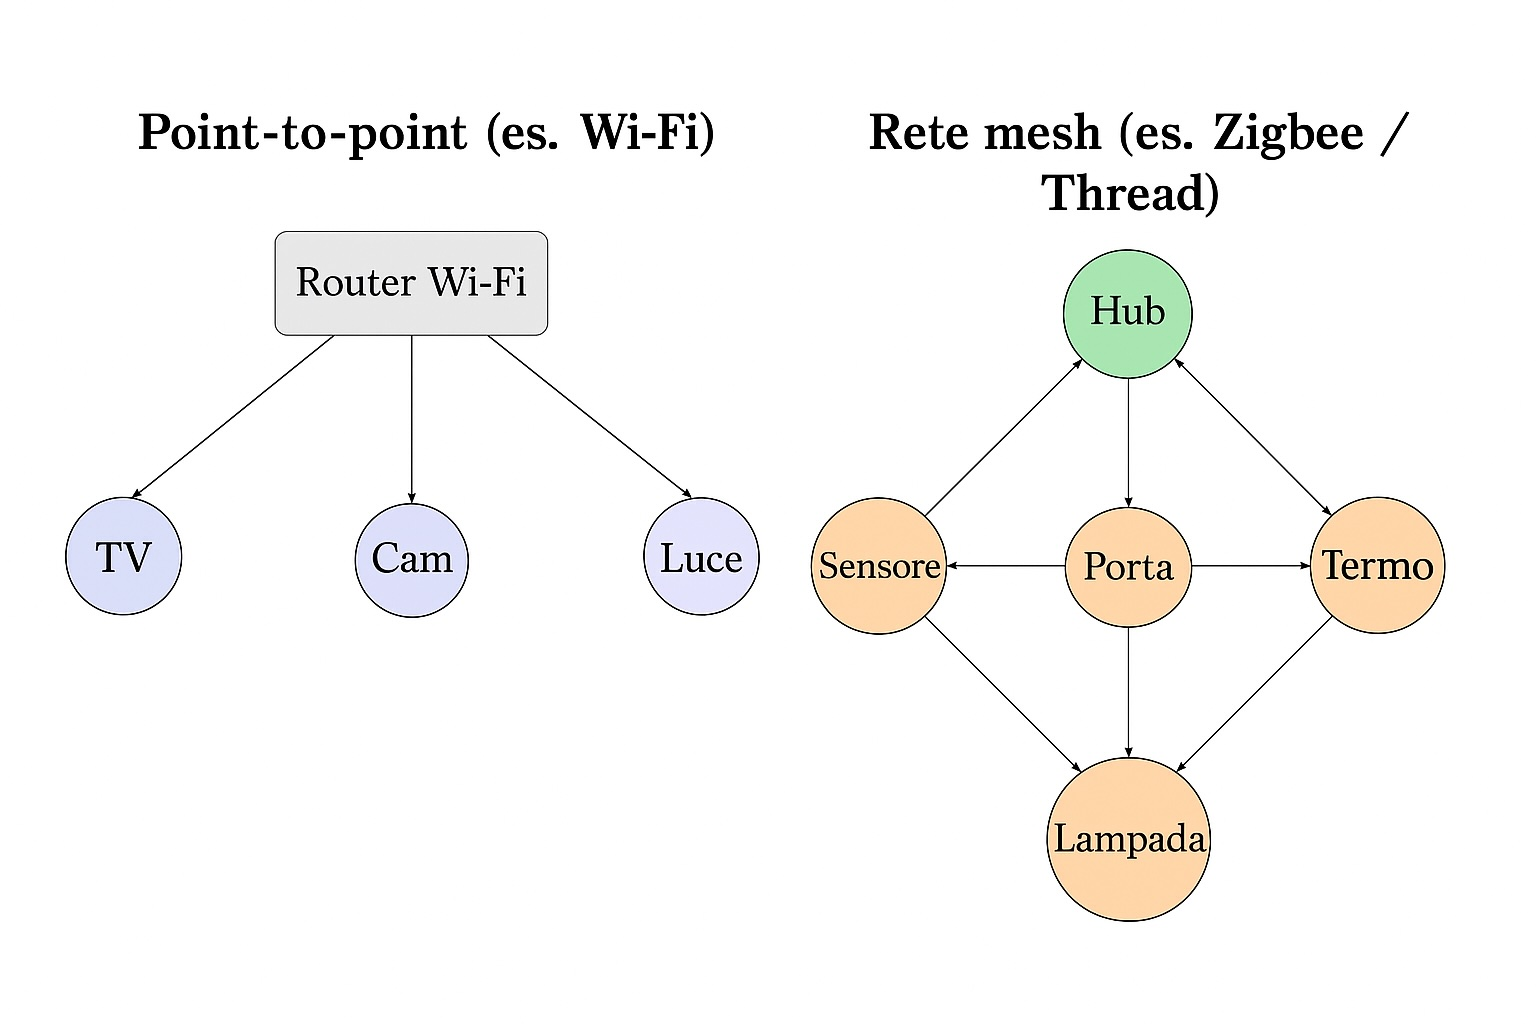
\includegraphics[scale=0.3]{immagini/reti.jpeg}
    \caption{Interfaccia Apple Home con dispositivi configurati}
    \label{fig:reti-mesh}
\end{figure}

\end{comment}

\clearpage
\vspace*{2cm}
\begin{figure}[htbp]
\centering
\begin{tikzpicture}[
  node distance=1.8cm and 2.5cm,
  every node/.style={font=\small},
  mesh/.style={draw, fill=orange!20, circle, minimum size=1.2cm},
  wifi/.style={draw, fill=blue!10, circle, minimum size=1.2cm},
  hub/.style={draw, fill=green!20, rounded corners, minimum width=2.5cm, minimum height=1cm},
  router/.style={draw, fill=gray!20, rounded corners, minimum width=2.5cm, minimum height=1cm}
]

% Titoli
\node[draw=none] at (0,8) {\textbf{Point-to-point (es. Wi-Fi)}};
\node[draw=none] at (10,8) {\textbf{Rete mesh (es. Zigbee / Thread)}};

% Wi-Fi Section
\node[router] (router) at (0,6.5) {Router Wi-Fi};

\node[wifi] (tv) at (-2,4.8) {TV};
\node[wifi] (cam) at (0.5,4.8) {Cam};
\node[wifi] (light1) at (2,4.8) {Luce 1};
\node[wifi] (light2) at (-2,3) {Luce 2};
\node[wifi] (thermo) at (-0.4,3) {Termo};
\node[wifi] (blind) at (2,3) {Finestra};

\draw[-{Latex}] (router) -- (tv);
\draw[-{Latex}] (router) -- (cam);
\draw[-{Latex}] (router) -- (light1);
\draw[-{Latex}] (router) -- (light2);
\draw[-{Latex}] (router) -- (thermo);
\draw[-{Latex}] (router) -- (blind);

% Mesh Section
\node[hub] (hub) at (10,6.5) {Hub};

\node[mesh] (sensor) at (8,4.8) {Sensore};
\node[mesh] (door) at (10,4.8) {Porta};
\node[mesh] (thermoM) at (12,4.8) {Termo};

\node[mesh] (lamp) at (9,3) {Lampada};
\node[mesh] (lightM) at (11,3) {Luce 2};
\node[mesh] (blind1) at (8.5,0.8) {Finestra 1};
\node[mesh] (blind2) at (11.5,0.8) {Finestra 2};

% Hub links
\draw[-{Latex}] (hub) -- (sensor);
\draw[-{Latex}] (hub) -- (door);
\draw[-{Latex}] (hub) -- (thermoM);

% Mesh links
\draw[<->]  (sensor) -- (lamp);
\draw[<->]  (sensor) -- (lightM);
\draw[<->]  (door) -- (lamp);
\draw[<->]  (door) -- (thermoM);
\draw[<->]  (lamp) -- (blind1);
\draw[<->]  (lightM) -- (blind2);
\draw[<->]  (lamp) -- (lightM);
\draw[<->]  (blind1) -- (blind2);
\draw[<->]  (thermoM) -- (blind2);

\end{tikzpicture}
\caption{Confronto tra rete point-to-point (Wi-Fi) e rete mesh (Zigbee/Thread).}
\label{fig:smart-home-mesh-vs-wifi}
\end{figure}



In definitiva, quando si progettano sistemi domotici destinati a durare nel tempo e ad adattarsi a contesti mutevoli, scegliere protocolli con meccanismi di recupero e adattamento diventa una garanzia di stabilità e continuità.

\section{Confronto prestazionale tra Zigbee, Z-Wave, Wi-Fi, Thread e Matter}

\subsection{Zigbee: il veterano delle reti mesh}

Zigbee è considerato uno dei protocolli più consolidati nell’ambito della domotica, grazie alla sua lunga presenza sul mercato e alla vasta adozione da parte dei produttori. Basato sullo standard IEEE 802.15.4, opera principalmente sulla banda a 2.4 GHz, la stessa condivisa con Wi-Fi e Bluetooth.

\textbf{Punti di forza:}
\begin{itemize}
    \item Ecosistema maturo con ampia disponibilità di dispositivi
    \item Supporto per reti mesh auto-riparanti fino a 65.000 nodi teorici
    \item Profili applicativi standardizzati (es. Zigbee Home Automation, Zigbee Light Link)
    \item Consumi energetici estremamente ridotti
\end{itemize}

\textbf{Limitazioni:}
\begin{itemize}
    \item Rischio di interferenze nella banda 2.4 GHz
    \item Complessità nella gestione di reti molto estese
    \item Frammentazione tra profili e versioni differenti
    \item Velocità non adatta a trasferimenti di dati intensivi
\end{itemize}

Philips Hue, ad esempio, utilizza Zigbee per controllare fino a 50 lampadine con un singolo bridge, offrendo sincronizzazione precisa e latenza impercettibile.

\subsection{Z-Wave: l'alternativa su frequenze dedicate}

Z-Wave si distingue per l’utilizzo di frequenze sub-GHz (868 MHz in Europa, 908 MHz negli USA), che garantiscono una maggiore penetrazione attraverso muri e ridotte interferenze rispetto alla banda 2.4 GHz.

\textbf{Caratteristiche distintive:}
\begin{itemize}
    \item Interoperabilità certificata tra dispositivi Z-Wave
    \item Portata estesa fino a 100 metri in campo aperto
    \item Topologia mesh con routing source-routed ottimizzato
    \item Limite di 232 nodi per rete, sufficiente per l’ambito residenziale
\end{itemize}

La sua velocità massima, pari a 100 kbps, lo rende inadatto a carichi di dati elevati, ma perfetto per sistemi di controllo. Un impianto di sicurezza domestica può includere sensori di movimento, contatti magnetici per porte/finestre e sirene ad alta affidabilità.

\subsection{Wi-Fi: potenza e versatilità}

Il Wi-Fi domina per capacità di banda e diffusione. La presenza capillare di router domestici riduce la necessità di infrastrutture dedicate, rendendolo ideale per dispositivi che richiedono elevato throughput.

\textbf{Vantaggi competitivi:}
\begin{itemize}
    \item Larghezza di banda elevatissima, adatta a video e trasferimenti intensivi
    \item Infrastruttura già presente nella maggior parte delle abitazioni
    \item Supporto IP nativo, ideale per integrazione cloud
    \item Ottimizzazioni recenti in Wi-Fi 6 per dispositivi IoT (es. Target Wake Time)
\end{itemize}

\textbf{Sfide operative:}
\begin{itemize}
    \item Consumo energetico elevato, inadatto a dispositivi a batteria
    \item Degrado prestazionale con molti dispositivi connessi a un singolo access point
    \item Latenza variabile in presenza di congestione di rete
    \item Hardware più costoso rispetto ad alternative low-power
\end{itemize}

Le videocamere IP rappresentano un'applicazione ideale: richiedono banda elevata e sono alimentate da rete elettrica, eliminando il vincolo energetico \cite{WiFiVsIoT}.

\subsection{Thread: l'evoluzione IP-native}

Thread è un protocollo mesh moderno progettato per supportare IPv6 nativamente, con un’architettura leggera e sicura adatta all’era dell’interoperabilità e del cloud.

\textbf{Innovazioni chiave:}
\begin{itemize}
    \item Supporto IPv6 nativo con instradamento end-to-end
    \item Sicurezza avanzata con crittografia AES e gestione automatica delle chiavi
    \item Commissioning semplice via smartphone
    \item Mesh self-healing con tempi di riconvergenza rapidi
\end{itemize}

Le sue latenze sono paragonabili a Zigbee (20–50 ms), ma con un’architettura più moderna e scalabile. Dispositivi come Apple HomePod mini o Google Nest Hub fungono da border router per reti Thread, facilitando l’adozione senza componenti aggiuntivi \cite{thread-spec}.

\subsection{Matter: l’unificatore dell’ecosistema}

Matter si propone come livello applicativo universale, operando sopra protocolli esistenti come Thread, Wi-Fi ed Ethernet. Il suo obiettivo è garantire interoperabilità trasparente tra piattaforme e produttori.

\textbf{Punti di forza:}
\begin{itemize}
    \item Compatibilità trasversale tra Apple, Google, Amazon, Samsung
    \item Sicurezza integrata nel design, con certificazione obbligatoria
    \item Commissioning tramite QR code o NFC
    \item Comunicazione locale senza necessità di cloud
\end{itemize}

Matter introduce un overhead minimo (circa 5–10\% di latenza aggiuntiva), ma il vantaggio in termini di compatibilità compensa ampiamente. Un termostato compatibile può essere gestito indistintamente da Siri, Google Assistant o Alexa, mantenendo la stessa qualità d’interazione \cite{MatterWhitePaper}.

\begin{table}[htbp]
\centering
\begin{tabular}{|l|c|c|c|c|c|}
\hline
\textbf{Parametro} & \textbf{Zigbee} & \textbf{Z-Wave} & \textbf{Wi-Fi} & \textbf{Thread} & \textbf{Matter} \\
\hline
Banda & 2.4 GHz & Sub-GHz & 2.4/5 GHz & 2.4 GHz & - \\
Topologia & Mesh & Mesh & Point-to-point & Mesh & - \\
Velocità max & 250 kbps & 100 kbps & \textgreater100 Mbps & 250 kbps & - \\
Energia & Molto bassa & Bassa & Alta & Bassa & Variabile \\
Interoperabilità & Limitata & Alta (cert.) & Variabile & Alta & Massima \\
\hline
\end{tabular}
\caption{Confronto sintetico tra protocolli e standard IoT in ambito domotico}
\label{tab:confronto-protocolli}
\end{table}

\section{Scalabilità dei protocolli in ambienti domestici complessi}

Man mano che le abitazioni intelligenti si arricchiscono di sensori, attuatori e dispositivi di controllo, il tema della \textbf{scalabilità} diventa centrale. Un sistema domotico moderno non si limita più ad accendere qualche luce o a regolare il termostato: può arrivare a gestire centinaia di elementi distribuiti in ambienti ampi e strutturati. In questo contesto, è fondamentale comprendere come i principali protocolli IoT reagiscano all’aumento della complessità della rete.

\subsection{Scalabilità per protocollo}

\subsubsection{Zigbee: tra teoria e realtà}

Zigbee dichiara il supporto fino a 65.000 dispositivi per rete, un numero che, sulla carta, garantirebbe ampie possibilità di espansione. Tuttavia, in ambito residenziale, questa soglia è ben lontana dalla realtà operativa.

Già superata la soglia dei 200-300 dispositivi, cominciano a emergere difficoltà pratiche:
\begin{itemize}
    \item Latenze maggiori dovute al routing tra nodi multipli
    \item Congestione nella banda a 2.4 GHz, soprattutto in ambienti densi
    \item Rallentamenti durante aggiornamenti firmware distribuiti
    \item Complessità crescente nella configurazione e manutenzione
\end{itemize}

Una strategia spesso adottata è la creazione di \textbf{sotto-reti logiche} distinte, ciascuna gestita da un coordinator dedicato, per esempio separando l’illuminazione dalla climatizzazione o dai sistemi di sicurezza.

\subsubsection{Z-Wave: solido entro i propri limiti}

Z-Wave ha un limite teorico molto più contenuto: 232 dispositivi per rete. Tuttavia, per la maggior parte delle abitazioni — anche quelle di grandi dimensioni — si tratta di un numero più che sufficiente. La gestione più semplice e il minor rischio di congestione radio, grazie all’uso della banda sub-GHz, lo rendono una scelta solida e prevedibile.

Un'abitazione con circa 100 dispositivi (tra interruttori, sensori e attuatori) rientra tranquillamente nei limiti del protocollo, offrendo ancora margine per ulteriori espansioni.

\subsubsection{Thread e Matter: progettati per crescere}

Thread è stato pensato fin dall’inizio per reti scalabili, affidabili e facilmente gestibili:
\begin{itemize}
    \item I router mesh distribuiti bilanciano il traffico in modo dinamico
    \item L'uso nativo di IPv6 semplifica il routing e la gestione
    \item La rete si auto-configura e auto-ripara in caso di guasti
\end{itemize}

Test su installazioni reali mostrano che anche con oltre 200 dispositivi, i tempi di risposta restano sotto i 100 ms nel 95° percentile, con una degradazione molto graduale delle prestazioni all’aumentare del carico.

Matter, appoggiandosi a Thread (e in parte al Wi-Fi), eredita e potenzia questa capacità, offrendo al tempo stesso interoperabilità tra ecosistemi e gestione centralizzata semplificata.

\subsection{Strategie di progettazione per reti complesse}

\subsubsection{Progettare la rete per livelli}

Quando i dispositivi aumentano, progettare in modo gerarchico diventa essenziale. Una buona architettura divide la rete in tre livelli logici:

\begin{enumerate}
    \item \textbf{Livello Edge}: i dispositivi periferici (sensori, attuatori) che eseguono compiti specifici
    \item \textbf{Livello di Aggregazione}: hub locali o controller di zona che raccolgono e instradano i dati
    \item \textbf{Livello Core}: un controller principale (o cloud gateway) che integra, elabora e coordina tutto il sistema
\end{enumerate}

Questa suddivisione migliora la stabilità, semplifica la manutenzione e consente di isolare eventuali malfunzionamenti, evitando che si propaghino all’intero sistema.

\subsubsection{Separare per funzione: la rete è più leggibile}

Un'altra strategia efficace è la suddivisione dei dispositivi in reti logiche in base alla loro funzione:

\begin{itemize}
    \item \textbf{Rete Sicurezza}: dispositivi critici come sensori di movimento, allarmi e serrature (dove l'affidabilità è prioritaria)
    \item \textbf{Rete Comfort}: luci, termostati e tapparelle (ottimizzati per reattività e basso consumo)
    \item \textbf{Rete Media}: smart TV, speaker, videocamere (dove la banda e la connessione stabile sono fondamentali)
\end{itemize}

In questo modo si ottimizzano i protocolli per ciascun gruppo: Z-Wave può essere usato per la sicurezza, Zigbee o Thread per l’illuminazione, e il Wi-Fi per streaming e intrattenimento.

\subsection{Conclusioni sulla scalabilità}

In sostanza quando ci troviamo a realizzazione di sistemi domotici complessi, la prima vera sfida è quella della scalabilità che non si esaurisce nei soli numeri dichiarati dai produttori. Al contrario, deve essere fondamentale che la rete sia in grado di mantenere buoni tempi di risposta, sia semplice nella gestione ed affidabilità, sopratutto  quando il numero di dispositivi collegati aumenta sensibilmente.\\

Ogni protocollo che abbiamo visto finoea presenta caratteristiche diverse in questo scenario.\\
Zigbee può scalare bene, ma richiede una buona esperienza nella progettazione di rete per evitare colli di bottiglia.\\
Z-Wave, per la sua semplicità di configurazione e la sua stabilità, ottenuta sfruttando le banda sub-GHz con meno traffico, si adatta perfettamente a contesti residenziali di dimensioni medio-piccole.\\
Thread e Matter, diversamente dai precedenti, offrono un approccio più moderno e flessibile, risultando particolarmente indicati per installazioni più grandi, complesse e in continua evoluzione, spinto anche dall'innovazione che le proncipali aziende stanno dando a questo protocollo.\\

In conclusione, per definire il successo di una rete domotica complessa e grande, non bisogna guardare solo dal protocollo che abbiamo scelto, ma soprattutto da come viene disegnata: una buona progettazione, cola presenza di segmentazioni funzionali, la definizione di una organizzazione gerarchica, consentono di ottenere risultati affidabili e duraturi, qualunque sia la tecnologia utilizzata.
